\documentclass{standalone}

\usepackage{lscape}
%Math typesetting packages
\usepackage{amsfonts, amssymb, amsmath, latexsym, amsthm,xparse, bm}
\newcommand\simiid{\stackrel{iid}{\sim}}
\newcommand\simind{\stackrel{ind}{\sim}}
\NewDocumentCommand{\qfrac}{smm}{%
  \dfrac{\IfBooleanT{#1}{\vphantom{\big|}}#2}{\mathstrut #3}%
}

\usepackage{tikz}
\usetikzlibrary{calc,arrows,positioning,shapes,shapes.gates.logic.US,trees, intersections}

\begin{document}

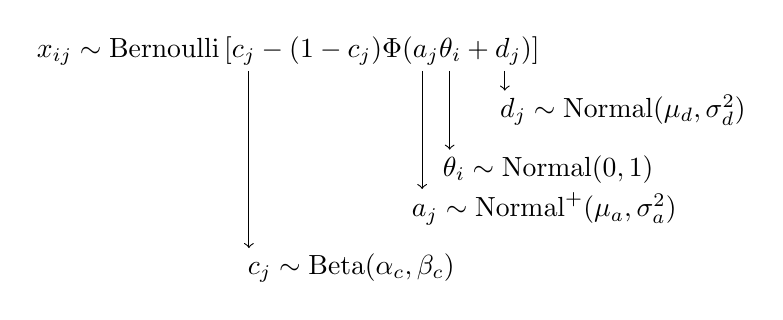
\begin{tikzpicture}
  \node at (0,0) {$x_{ij} \sim \mathrm{Bernoulli}\left[c_j - (1-c_j)\Phi(a_j \theta_i + d_j)\right]$} ;
  	\draw[->] (2.75, -0.25) -- (2.75, -0.5);
  	\node at (4.25, -0.75) {$d_{j}\sim \mathrm{Normal}(\mu_{d}, \sigma^2_{d})$};
  	\draw[->] (2.05,-0.25) -- (2.05,-1.25);
  	\node at (3.3, -1.5) {$\theta_i \sim \mathrm{Normal}(0,1)$};
  	\draw[->] (1.7,-0.25) -- (1.7,-1.75);
  	\node at (3.25, -2) {$a_j\sim \mathrm{Normal}^{+}(\mu_a, \sigma^2_a)$};
  	\draw[->] (-0.5, -0.25) -- (-0.50, -2.5);
  	\node at (0.8, -2.75) {$c_j \sim \mathrm{Beta}(\alpha_c,\beta_c)$};  		
\end{tikzpicture}

\end{document}